\section{Rancangan Solusi}
\label{sec:rancangan-solusi}

Dengan segala kebutuhan yang sudah dianalisis, maka akan dibuat beberapa komponen penyusun sistem yang bisa dilihat pada gambar \ref{fig:rancangan-sistem}. Rencananya, sistem kontrol fleksibel akan dikembangkan dari luar kubernetes cluster sedangkan \textit{Elastic Search} itu sendiri diletakkan didalam kubernetes. Integrasi dengan API \textit{Elastic Search} akan melalui \textit{service} yang disediakan kubernetes sedangkan untuk mengontrol kubernetesnya sendiri akan digunakan \textit{Kubernetes Client Library}.

\begin{figure}[h]
    \centering
    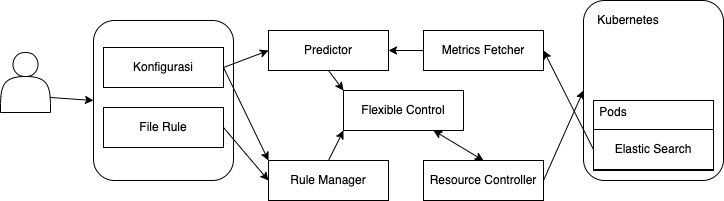
\includegraphics[width=0.8\textwidth]{chapter-3/rancangan.png}
    \caption{Rancangan Komponen Penyusun Sistem}
    \label{fig:rancangan-sistem}
\end{figure}

Pada gambar \ref{fig:rancangan-sistem}, sistem kontrol fleksibel tersusun dari beberapa komponen, diantaranya sebagai berikut.

\begin{enumerate}
    \item \textbf{Konfigurasi dan \textit{File Rule}}
    
    Konfigurasi dan \textit{File Rule} akan berinteraksi langsung dengan pengguna. Konfigurasi akan dibaca oleh mayoritas komponen sebagai pengaturan terhadap sistem sedangkan file rule yang di\textit{parse} oleh \textit{rule manager} untuk mengatur trigger dari \textit{resource controller} melakukan kontrol fleksibel terhadap alokasi sumber daya.

    \item \textbf{Kubernetes dan \textit{Elastic Search}}
    
    \textit{Elastic Search} akan diletakkan pada sebuah \textit{pods} di dalam sebuah \textit{cluster Kubernetes}. Dibuatkan sebuah \textit{service} agar \textit{Elastic Search} dapat diakses dari luar \textit{cluster}.
    
    \item \textbf{\textit{Predictor}}
    
    \textit{Predictor} akan berisikan model ARIMA untuk setiap variabel yang telah ditentukan. Model-model ini akan digunakan untuk memprediksi nilai variabel pada waktu selanjutnya sesuai permintaan \textit{rule manager}. Karena setiap rule mungkin untuk memiliki keperluan data untuk waktu prediksi yang berbeda.

    \item \textbf{\textit{Metrics Fetcher}}
    
    Komponen \textit{Metrics Fetcher} bertugas untuk menembak \href{https://www.elastic.co/guide/en/elasticsearch/reference/current/cluster-nodes-stats.html}{\textit{Node Stats API}} yang dimiliki oleh \textit{Elastic Search} dan meneruskannya kepada komponen \textit{Predictor} untuk melatih model.

    \item \textbf{\textit{Rule Manager}}
    
    Komponen \textit{Rule Manager} akan melakukan parsing terhadap file rule yang telah diisi oleh pengguna dan mengatur \textit{trigger}. Selain itu, komponen ini akan memberikan informasi tentang waktu prediksi yang diperlukan berdasarkan \textit{rule} yang telah dibuat oleh pengguna.

    \item \textbf{\textit{Resource Controller}}
    
    Komponen \textit{Resource Controller} akan memanfaatkan \textit{Kubernetes Client Library} untuk mengubah spesifikasi \textit{deployment} sehingga alokasi sumber daya dapat berubah. Pada pembuatan komponen ini, harus dilakukan eksperimen \textit{In-place Resource Resize} untuk mengubah alokasi sumber daya tanpa melakukan \textit{restart}.

    \item \textbf{\textit{Adaptive Control}}
    
    Komponen \textit{Adaptive Control} adalah komponen \textit{high-level} yang akan mengintegrasikan dan mengkolaborasikan komponen-komponen yang disebutkan sebelumnya.
\end{enumerate}